\documentclass[10pt]{article}

% \usepackage{times}
\usepackage{amsmath}
\usepackage{amssymb}

\usepackage{amsthm}
\theoremstyle{plain}
\newtheorem{definition}{Definition}
\newtheorem{corollary}{Corollary}
\newtheorem{proposition}{Proposition}
\newtheorem{lemma}{Lemma}

\usepackage{txfonts}

\usepackage[en-GB]{datetime2}
\DTMlangsetup[en-GB]{ord=omit}

\usepackage{url}
\urlstyle{rm}

\usepackage[ruled,vlined,linesnumbered]{algorithm2e}
\SetKwFor{ForEach}{for each}{do}{end}
\SetKwProg{Function}{function}{}{}
\SetKwProg{Procedure}{procedure}{}{}
\SetKwProg{Class}{class}{}{}
\SetKwInput{Persistent}{persistent}{}{}
\SetKwInput{Input}{input}{}{}
\SetKwIF{WithProbability}{}{Else}{with probability}{do}{}{else}{end with}
\SetKw{Break}{break}
\DontPrintSemicolon

\usepackage{graphicx}

\usepackage{bm}
\newcommand{\vect}[1]{\bm{#1}}

\usepackage{forest}
\usepackage{subcaption}

\DeclareMathOperator*{\argmax}{\arg\!\max}
\DeclareMathOperator*{\argmin}{\arg\!\min}
\DeclareMathOperator*{\arctantwo}{arctan2}

\usepackage{mdframed}
\usepackage{xcolor}
\newenvironment{note}[1][Note]{
    \begin{center}
    	\begin{minipage}{0.9\linewidth}
    		\begin{mdframed}[backgroundcolor=yellow!25,linewidth=0pt]
    			\textbf{#1:} }{
    		\end{mdframed}
    	\end{minipage}
    \end{center}
}

\usepackage{booktabs}

\usepackage{pifont}
\newcommand{\cmark}{\ding{51}}
\newcommand{\xmark}{\ding{55}}

\usepackage{tikz}
\usetikzlibrary{calc}

\DeclareFontFamily{U}{mathx}{\hyphenchar\font45}
\DeclareFontShape{U}{mathx}{m}{n}{<5> <6> <7> <8> <9> <10> <10.95> <12> <14.4> <17.28> <20.74> <24.88> mathx10}{}
\DeclareSymbolFont{mathx}{U}{mathx}{m}{n}
\DeclareMathSymbol{\bigtimes}{1}{mathx}{"91}

\usepackage{pdflscape}

\title{Simulator-Based Verification of Autonomous Vehicles: Agent-Based Test Generation}
\author{}
\date{\DTMcurrenttime, \today}

\begin{document}

\maketitle

\section{Introduction}

\begin{itemize}
    \item \textbf{Time} is implicit and discrete, with agents choosing actions at each timestep, and a time resolution constant specifying the simulation time between timesteps
    \item \textbf{State space} is continuous and feature-based techniques are probably more effective than discretisation
    \item \textbf{Actions} may be multi-body and/or multi-effector
    \item \textbf{Action space} is continuous and discretisation typically requires durative actions
    \item \textbf{Observability} is full, meaning that a sensor model is not required (although partial observability can be simulated)
    \item \textbf{Initial state} may be given (meaning a partial policy is sufficient) or may not be given (meaning a complete policy is necessary)
    \item \textbf{Objectives} are goals states with transition costs/rewards, meaning in general that the horizon is indefinite, but a finite-horizon may also be imposed
    \item \textbf{Model} for transitions and objectives is unknown, but can be sampled through interaction with a simulator
    \item \textbf{Game} involving two or more players (agents), including a potentially adversarial design under verficiation (i.e.\ the ego agent)
\end{itemize}

\newpage
\section{Preliminaries}
We rely on some standard mathematical notation:
$v_{i}$ is an element of vector $\vect{v} = (v_{1}, \dots, v_{n})$ with $\vect{v}_{-i} = (v_{1}, \dots, v_{i-1}, v_{i+1}, \dots, v_ {n})$ the subvector of $\vect{v}$ excluding~$v_{i}$,
$|S|$ is the cardinality of set $S$,
$2^{S}$ is the powerset of $S$,
$\Delta(S)$ is the set of probability distributions over $S$,
$\mathbb{R}$ is the set of real numbers with $\mathbb{R}^{\ge 0}$ the subset of non-negative real numbers,
% $\mathbb{Z}^{\ge 0}$ is the set of non-negative integers,
and $\mathbb{N}$ is the set of natural numbers.
A function $f : X \to Y$ is a surjection if for each $y \in Y$ there exists some $x \in X$ such that $f(x) = y$.
Given a function $f : X \to Y$, the inverse image of function $f$ is a function $f_{B,N}^{-1} : Y \to 2^{X}$ defined for each $y \in Y$ as $f_{B,N}^{-1}(y) = \{ x \in X \mid f(x) = y \}$.

% \subsection{Normal-Form Games}
% An ($n$-player) normal-form game is a tuple $(N, A, \vect{u})$ where $N = \{ 1, \dots, n \}$ is a finite set of players, $A = A_{1} \times \dots \times A_{n}$ is a set of action profiles with $A_{i}$ the (possibly infinite) set of actions available to player $i \in N$, and $\vect{u} = (u_{1}, \dots, u_{n})$ is a profile of utility functions with $u_{i} : A \to \mathbb{R}$ the utility function for~$i$.
% A (mixed) strategy for player $i \in N$ is a probability distribution $\psi \in \Delta(A_{i})$ with $\vect{\psi} \in \Delta(A_{1}) \times \dots \times \Delta(A_{n})$ a (mixed) strategy profile.
% A strategy $\psi$ for player $i \in N$ is a pure strategy if $\psi(a) = 1$ for some $a \in A_{i}$.
% A strategy profile $\vect{\psi}$ is a pure strategy profile if $\psi_{i}$ is a pure strategy for each $i \in N$.
% For convenience, we may denote a pure strategy $\psi$ for player $i \in N$ directly by the action $a \in A_{i}$ such that $\psi(a) = 1$.
% Likewise, we may denote a pure strategy profile $\vect{\psi}$ directly by the action profile $\vect{a} \in A$ such that $\psi_{i}(a_{i}) = 1$ for each player $i \in N$.
% The expected utility of a strategy profile $\vect{\psi}$ is defined as:
% \begin{equation*}
% 	u_{i}(\vect{\psi}) = \sum_{\vect{a} \in A} u_{i}(\vect{a}) \prod_{j \in N} \psi_{j}(a_{j})
% \end{equation*}
%
% In game theory, a solution concept is a prediction of how a game will be played.
% Solution concepts are typically based on the idea that each player will try to maximise their expected utility under the assumption that other players will do the same.
% A feasible deviation from strategy profile $\vect{\psi}$ by player $i \in N$ is a strategy profile $\vect{\psi'} = (\vect{\psi}_{-i}, \psi')$ where $\psi'$ is a strategy for $i$.
% A strategy profile $\vect{\psi}$ is a Nash equilibrium if no player $i \in N$ has a feasible deviation $\vect{\psi'}$ from $\vect{\psi}$ such that $u_{i}(\vect{\psi'}) > u_{i}(\vect{\psi})$.
% Every normal-form game with a finite set of action profiles is guaranteed to have at least one (not necessarily pure) Nash equilibrium~\cite{Nash:AM:1951}.
% A Nash equilibrium is also guaranteed to exist for certain classes of normal-form game with an infinite set of action profiles~\cite{}.
%
% \subsection{Markov Games}
% A (fully observable) Markov game is a tuple $(N, S, A, T, \vect{R})$ where
% $N = \{ 1, \dots, n \}$ is a finite set of players,
% $S$ is a (possibly infinite) set of states,
% $A = A_{1} \times \dots \times A_{n}$ is a set of action profiles with $A_{i}$ the (possibly infinite) set of actions available to player $i \in N$,
% $T : S \times A \to \Delta(S)$ is a (stochastic) transition function, and
% $\vect{R} = (R_{1}, \dots, R_{n})$ is a profile of reward functions with $R_{i} : S \times A \times S \to \mathbb{R}$ the reward function for player $i \in N$.
% A Markov game is zero-sum if $\sum_{i \in N} R_{i}(s, \vect{a}, s') = 0$ for each $\vect{a} \in A$ and all $s, s' \in S$.
%
% Markov games (also known as stochastic games~\cite{Shapley:PNAS:1953}) are composed of a sequence of normal-form games, called stage games, where players seek to optimise their return for the whole game rather than for individual stage games.
% The current stage game is determined by the current state, and players transition between states by executing actions simultaneously.
% The game is said to be fully observable because players are assumed to observe the current (shared) state at each decision step.
% Let $T(s, \vect{a}, s')$ denote the probability of transitioning to state $s' \in S$ after executing action profile $\vect{a} \in A$ in state $s \in S$ according to probability distribution $T(s, \vect{a})$.
% The probability of transitioning to state $s' \in S$ after executing strategy profile $\vect{\psi}$ in state $s \in S$ is:
% \begin{equation*}
%     T(s, \vect{\psi}, s') = \prod_{\vect{a} \in A} T(s, \vect{a}, s') \prod_{j \in N} \psi_{j}(a_{j})
% \end{equation*}
% The stage game for state $s \in S$ is a normal-form game $(N, A, \vect{u})$ where the utility function $u_{i}$ for player $i \in N$ is defined for each action profile $\vect{a} \in A$ as the immediate expected reward:
% \begin{equation*}
%     u_{i}(\vect{a}) = \sum_{s' \in S} T(s, \vect{a}, s') R_{i}(s, \vect{a}, s')
% \end{equation*}
% Markov games subsume numerous other frameworks, including repeated games when $|S| = 1$, and Markov decision processes (MDPs) when $|N| = 1$.
%
% Solutions to Markov games are represented as functions, called policies, that map \emph{histories} to strategies.
% An execution is a possibly infinite sequence of states and action profiles $(s_{1}, \vect{a}_{1}, s_{2}, \vect{a}_{2}, \dots)$.
% A history of length $t$ is a finite execution $h_{t} = (s_{1},a_{1},$ $\dots, a_{t-1}, s_{t})$ ending in a state.
% Let $H_{t}$ be the set of histories of length $t$ with $D = \{ 1, 2, \dots, t_{\max} \}$ the set of decision-steps up to horizon $t_{\max} \in \mathbb{N} \cup \{ \infty \}$ and $H = \{ h \in H_{t} \mid t \in D \}$ the set of histories up to $t_{\max}$.
% A (stochastic or mixed) policy for player $i \in N$ is a function $\pi_{i} : H' \to \Delta(A_{i})$ where $H' \subseteq H$.
% Let $\pi_{i}(h, a)$ denote the probability that player $i \in N$ should execute action $a \in A_{i}$ in history $h \in H'$ according to strategy $\pi_{i}(h)$.
% A policy $\pi_{i}$ for player $i \in N$ is a complete policy if $H' = H$, otherwise $\pi_{i}$ is a partial policy.
% A policy $\pi_{i}$ for player $i \in N$ is a deterministic (or pure) policy if $\pi_{i}(h, a) = 1$ for each $h \in H'$ and some $a \in A_{i}$.
% For convenience, we may denote a pure policy $\pi_{i}$ for player $i \in N$ directly by a policy $\pi_{i}' : H' \to A$ where $\pi_{i}'(h) = a$ such that $\pi_{i}(h, a) = 1$.
% A policy $\pi_{i}$ for player $i \in N$ is Markovian if $\pi_{i}(h_{t}) = \pi_{i}(h_{t'})$ for all $h_{t}, h_{t'} \in H'$ such that $t = t'$ and $s_{t} = s_{t'}$.
% A Markovian policy for player $i \in N$ may be written as $\pi_{i} : X \to \Delta(A_{i})$ where $X \subseteq S \times D$.
% A Markovian policy $\pi_{i}$ for player $i \in N$ is a stationary policy if $\pi_{i}(s, t) = \pi_{i}(s, t')$ for all $(s, t), (s, t') \in X$, otherwise $\pi_{i}$ is a non-stationary policy.
% A stationary Markovian policy for player $i \in N$ may be written as $\pi_{i} : S' \to \Delta(A_{i})$ where $S' \subseteq S$.
% A tuple $\vect{\pi} = \left( \pi_{1}, \dots, \pi_{n} \right)$ is a policy profile over $H' \subseteq H$ if $\pi_{i}$ is a policy over $H'$ for each $i \in N$.
% The strategy profile for history $h \in H'$ according to policy profile $\vect{\pi}$ is $\vect{\pi}(h) = \left( \pi_{1}(h), \dots, \pi_{n}(h) \right)$.
%
% Solutions are only well-defined for certain classes of Markov game.
% Two common examples are finite-horizon Markov games and infinite-horizon (discounted reward) Markov games.
% A finite-horizon Markov game is a tuple $(\Gamma, t_{\max})$ where $\Gamma$ is a Markov game and $t_{\max} \in \mathbb{N}$ is a horizon.
% An infinite-horizon Markov game is a tuple $(\Gamma, \gamma)$ where $\Gamma$ is a Markov game and $\gamma \in [0, 1)$ is a discount factor.
% It is known that attention can be restricted to stationary Markovian policies in the case of infinite-horizon Markov games, and to non-stationary Markovian policies in the case of finite-horizon Markov games.
% Unless stated otherwise, we will assume hereafter that all policies are either stationary or non-stationary Markovian policies.
% For an infinite-horizon Markov game $(\Gamma, \gamma)$, the expected value of policy profile $\vect{\pi}$ for player $i \in N$ in state $s \in S$ is:
% \begin{equation*}
%     V_{i}(\vect{\pi}, s) = \sum_{s' \in S} T(s, \vect{\pi}(s), s') \left[ R_{i}(s, \vect{\pi}(s), s') + \gamma V_{i}(\vect{\pi}, s') \right]
% \end{equation*}
% For a finite-horizon Markov game $(\Gamma, t_{\max})$, the expected value of policy profile $\vect{\pi}$ for player $i \in N$ in state $s \in S$, with $t \in D \cup \{ 0 \}$ remaining decision-steps, is:
% \begin{align*}
%     V_{i}(\vect{\pi}, s, t) =
%     \begin{cases}
%         \sum\limits_{s' \in S} T(s, \vect{\pi}(s, t), s') \left[ R_{i}(s, \vect{\pi}(s, t), s') + V_{i}(\vect{\pi}, s', t-1) \right] & \text{if $t > 0$} \\
%         0 & \text{if $t = 0$}
%     \end{cases}
% \end{align*}
% A feasible deviation from policy profile $\vect{\pi}$ by player $i \in N$ is a policy profile $\vect{\pi'} = (\vect{\pi}_{-i}, \pi')$ where $\pi'$ is a policy for $i$.
% A policy profile $\vect{\pi}$ is a Nash equilibrium if no player $i \in N$ has a feasible deviation $\vect{\pi'}$ from $\vect{\pi}$ such that $V_{i}(\vect{\pi'}, h) \ge V_{i}(\vect{\pi}, h)$ for each $h \in H'$ and $V_{i}(\vect{\pi'}, h') > V_{i}(\vect{\pi}, h')$ for some $h' \in H'$.
%
% \begin{note}[To do]
%     Confirm that this definition of a Nash equilibrium is correct with respect to histories (or states, or time-indexed states).
% \end{note}

\subsection{SSP Games}
A tuple $(N, S, A, T, R, G)$ is a (fully observable, two-player, zero-sum) stochastic shortest path (SSP) game if
$N = \{ 1, 2 \}$ is a set of \textbf{players},
$S$ is a (possibly infinite) set of \textbf{states},
$A = A_{1} \times A_{2}$ is a set of \textbf{action profiles} with $A_{i}$ the (possibly infinite) set of \textbf{actions} available to player $i \in N$,
$G \subseteq S$ is a (possibly infinite) set of \textbf{goal states} for player $1$,
$T : S \times A \to \Delta(S)$ is a (stochastic) \textbf{transition function} such that $T(s, \vect{a}, s) = 1$ for each $s \in G$ and each $\vect{a} \in A$,
and $R : S \times A \times S \to \mathbb{R}$ is a \textbf{reward function} for player $1$ such that $R(s, \vect{a}, s') = 0$ for each $s \in G$, each $\vect{a} \in A$, and each $s' \in S$.
Let $T(s, \vect{a}, s')$ denote the probability of transitioning to state $s' \in S$ after executing action profile $\vect{a} \in A$ in state $s \in S$ according to probability distribution $T(s, \vect{a})$.
An \textbf{execution} is a possibly infinite sequence $(s_{1}, \vect{a}_{1}, s_{2}, \vect{a}_{2}, \dots)$ of states and action profiles.
A \textbf{history} of length $t$ is a finite execution $h_{t} = (s_{1}, a_{1}, \dots, a_{t-1}, s_{t})$ ending in a state.
Let $H_{t}$ be the set of histories of length $t$ with $D = \{ 1, 2, \dots, t_{\max} \}$ the set of decision-steps up to horizon $t_{\max} \in \mathbb{N} \cup \{ \infty \}$ and $H = \{ h \in H_{t} \mid t \in D \}$ the set of histories up to $t_{\max}$.

A (mixed) \textbf{strategy} for player $i \in N$ is a probability distribution $\psi \in \Delta(A_{i})$.
A strategy $\psi$ for player $i \in N$ is a \textbf{pure strategy} if $\psi(a) = 1$ for some $a \in A_{i}$.
A (mixed) \textbf{policy} for player $i \in N$ is a function $\pi_{i} : H \to \Delta(A_{i})$.
Let $\pi_{i}(h, a)$ denote the probability that player $i \in N$ will execute action $a \in A_{i}$ in history $h \in H$ according to strategy $\pi_{i}(h)$.
A policy $\pi_{i}$ for player $i \in N$ is \textbf{pure} if $\pi_{i}(h, a) = 1$ for each $h \in H$ and some $a \in A_{i}$.
A pure policy for player $i \in N$ may be written as $\pi_{i} : H \to A$.
A policy $\pi_{i}$ for player $i \in N$ is \textbf{Markovian} if $\pi_{i}(h) = \pi_{i}(h')$ for all $h, h' \in H$ such that $t = t'$ and $s = s'$ where $h$ ends in state $s \in S$ after $t \in D$ timesteps (resp.\ $h'$ ends in state $s' \in S$ after $t' \in D$ timesteps).
A Markovian policy for player $i \in N$ may be written as $\pi_{i} : S \times D \to \Delta(A_{i})$.
A Markovian policy $\pi_{i}$ for player $i \in N$ is \textbf{stationary} if $\pi_{i}(s, t) = \pi_{i}(s, t')$ for each $s \in S$ and all $t, t' \in D$, otherwise $\pi_{i}$ is \textbf{non-stationary}.
A stationary policy for player $i \in N$ may be written as $\pi_{i} : S \to \Delta(A_{i})$.

A \textbf{policy profile} is a tuple $\vect{\pi} = \left( \pi_{1}, \pi_{2} \right)$ where $\pi_{i}$ is a policy for player $i \in N$.
The (mixed) \textbf{strategy profile} for history $h \in H$ according to policy profile $\vect{\pi}$ is $\vect{\pi}(h) = \left( \pi_{1}(h), \pi_{2}(h) \right)$.
A strategy profile $\vect{\pi}(h)$ for history $h \in H$ is a \textbf{pure strategy profile} for $h$ if $\pi_{i}(h)$ is a pure strategy for each $i \in N$.
Let $\vect{\pi}(h, \vect{a}) = \prod_{i \in N} \pi_{i}(h, a_{i})$ be the probability that action profile $\vect{a} \in A$ will be executed in history $h \in H$ according to policy profile~$\vect{\pi}$.
The \textbf{expected value} of policy profile $\vect{\pi}$ for player $i \in N$ in history $h \in H$ is:
\begin{equation}
    V_{i}(\vect{\pi}, h) = \sum_{\vect{a} \in A} \vect{\pi}(h, \vect{a}) \sum_{s' \in S} T(s, \vect{a}, s') \left[ R_{i}(s, \vect{a}, s') + V_{i}(\vect{\pi}, [h, \vect{a}, s']) \right]
\end{equation}
where $h$ ends in state $s \in S$.
Standard notions of optimality are not well-defined in SSP games when $V_{i}(\vect{\pi}, h) = \infty$ for any history $h \in H$, or when $V_{i}(\vect{\pi}, h') = -\infty$ for each $h' \in H$.
For this reason, solution definitions typically rely on assumptions that the process will (eventually) terminate by reaching a goal state, ensuring finite expected value for a given policy profile.
Let $\mathbb{P}(s \mid h, \vect{\pi}, t)$ denote the probability of transitioning from history $h \in H$ to state $s \in S$ within $t \in \mathbb{N}$ timesteps by following policy profile $\vect{\pi}$.
A policy $\pi_{1}$ for player $1$ is \textbf{proper} at history $h \in H$ if there exists some $t \in \mathbb{N}$ such that:
\begin{equation}
    \mathbb{P}(G \mid h, \pi_{1}, \pi_{2}, t) = \sum_{s' \in G} \mathbb{P}(s' \mid h, \pi_{1}, \pi_{2}, t) = 1
\end{equation}
for any policy $\pi_{2}$ for player $2$, otherwise $\pi_{1}$ is \textbf{improper} at $h$.
A policy $\pi_{1}$ for player $1$ is proper if $\pi_{1}$ is proper at each history $h \in H$, otherwise $\pi_{1}$ is improper.\footnote{The notions of proper and improper policies are undefined for player $2$.}
An SSP game is \textbf{solvable} if
there exists a policy $\pi_{1}$ for player $1$ such that $\pi_{1}$ is proper
and $V(\pi_{1}', h) = -\infty$ for any (improper) policy $\pi_{1}'$ for player $1$ such that $\pi_{1}'$ is improper at history $h \in H$.
A policy $\pi_{i}^{*}$ for player $1$ in a solvable SSP game is an \textbf{expectiminimax} policy for player $1$ if $\pi_{i}^{*}$ satisfies:
\begin{equation}
    \argmin_{\vect{\pi}_{-i}} V_{i}(\pi_{i}^{*}, \vect{\pi}_{-i}, h) \ge \argmin_{\vect{\pi}_{-i}'} V_{i}(\pi_{i}', \vect{\pi}_{-i}', h)
\end{equation}
for each policy $\pi_{i}'$ for player $1$ and each history $h \in H$.
It is known that attention in SSP games can be restricted to stationary pure policies~\cite{}.

% \subsection{SSP$_{s_{1}}$ Games}
% A policy $\pi_{i}$ for player $i \in N$ is \textbf{complete} if $H' = H$, otherwise $\pi_{i}$ is \textbf{partial}.
% A policy $\pi_{i}$ for player $i \in N$ is \textbf{closed} at state $s_{1} \in S$ if for each $h \in H$ such that $h$ is reachable from $s_{1}$ by following $\pi_{i}$ and facing any opposing policy profile $\vect{\pi}_{-i}$, then $h \in H'$.

% \newpage
% \section{Time-Limited SSPs}
% A tuple $(S, A, T, R, G)$ is a (fully observable) stochastic shortest path MDP (SSP) if
% $S$ is a (possibly infinite) set of states,
% $A$ is a (possibly infinite) set of actions,
% $G \subseteq S$ is a (possibly infinite) set of goal states,
% $T : S \times A \to \Delta(S)$ is a (stochastic) transition function satisfying $T(s, a, s) = 1$ for each $s \in G$ and each $a \in A$,
% and $R : S \times A \times S \to \mathbb{R}$ is a reward function satisfying $R(s, a, s') = 0$ for each $s \in G$, each $a \in A$, and each $s' \in S$.
% In the setting of SSPs it is known that attention can be restricted to stationary policies~\cite{Bertsekas:book:1995}.
% Let $\mathbb{P}(s \mid h, \vect{\pi}, t)$ denote the probability of transitioning from history $h \in H$ to state $s \in S$ within $t \in \mathbb{N}$ timesteps by following policy $\pi$.
% A policy $\pi$ is proper at state $s \in S$ if:
% \begin{equation*}
%     \mathbb{P}(G \mid h, \pi, t) = \sum_{s' \in G} \mathbb{P}(s' \mid h, \pi, t) = 1
% \end{equation*}
% for each history $h \in H$ such that $h$ terminates at $s$, otherwise $\pi$ is improper at $s$.
% A policy $\pi$ is proper if $\pi$ is proper at each state $s \in S$, otherwise $\pi_{1}$ is improper.
% An SSP is solvable if
% (i) there exists a policy $\pi$ such that $\pi$ is proper
% and (ii) $V(\pi', s) = -\infty$ for any (improper) policy $\pi'$ such that $\pi'$ is improper at state $s \in S$.
% A typical method to guarantee condition (ii) is to require for all $s, s' \in S$ and each $a \in A$ that $R(s, a, s') = 0$ if $s \in G$, and $R(s, a, s') < 0$ otherwise.
% In other words, every transition from a non-terminal state has a positive cost, which has the effect of causing all improper (i.e.\ non-terminating) policies to accumulate infinite cost.
%
% A tuple $(S, A, T, R, G, s_{1})$ is a initialised SSP if
% $(S, A, T, R, G)$ is an SSP
% and $s_{1} \in S$ is an initial state.
% A policy $\pi : S' \to A$ is closed at $s_{1}$ if for each state $s \in S$ such that $s$ is reachable from $s_{1}$  following $\pi$ then $s \in S'$.
%
% \begin{definition}
%     A tuple $(S, A, T, R, G, E, s_{1})$ is a initialised SSP with terminal states if:
%     \begin{itemize}
%         \item $(S, A, T, R, G, s_{1})$ is an initialised SSP
%         \item $E \subseteq S$ is a (possibly infinite) set of terminal states
%         \item $T(s, a, s) = 1$ for each $s \in G \cup E$ and each $a \in A$
%         \item $R(s, a, s') = 0$ for each $s \in G \cup E$, each $a \in A$, and each $s' \in S$
%     \end{itemize}
% \end{definition}
%
% \begin{definition}
%     Let $(S, A, T, R, G, s_{1})$ be an initialised SSP and $t_{\max} \in \mathbb{N}$ be a horizon.
%     An initialised SSP with terminal states $(S', A, T', R', G', E, s_{1})$ is a time-limited SSP, denoted $(S, A, T, R, G, s_{1}, t_{\max})$, if:
%     \begin{itemize}
%         \item $D = \{ 1, \dots, t_{\max} \}$ is a set of decision steps (or timesteps)
%         \item $S' = S \times D$ is a set of states
%         \item $G' = G \times D$ is a set of goal states
%         \item $E = S \times \{ 0 \}$ is a set of terminal states
%         \item $T' : S' \times A \to \Delta(S')$ is a (stochastic) transition function such that for each $s \in S$ and each $a \in A$:
%             \begin{itemize}
%                 \item $T'([s, 0], a, [s, 0]) = 1$
%                 \item $T'([s, t], a, [s', t - 1]) = T(s, a, s')$ for each $s' \in S$ and each $t \in D \setminus \{ 0 \}$
%             \end{itemize}
%         \item $R' : S' \times A \times S' \to \mathbb{R}$ a reward function such that for each $s \in S$, each $t \in D$, and each $a \in A$:
%             \begin{itemize}
%                 \item $R'([s, 0], a, [s, t]) = 0$
%                 \item $R'([s', t'], a, [s, t]) = R(s', a, s)$ for each $s' \in S$ and each $t' \in D \setminus \{ 0 \}$
%             \end{itemize}
%     \end{itemize}
% \end{definition}
%
% It follows that if $\pi$ is a (stationary) proper policy for the time-limited SSP $(S', A, T',$ $R', G')$, then $\pi$ is also a (non-stationary) proper policy for the SSP $(S, A, T, R, G)$ where $\mathbb{P}(G \mid h_{1}, \pi, t_{\max}) = 1$ with $h_{1}$ the empty history.
% Thus, time-limited SSPs are a special case of SSPs that require non-stationary policies, but still rely on stationary transition and reward functions (with the exception of special terminal states in $S \times \{ 0 \}$, which are absorbing and accumulate no cost/reward).
% Despite their similarity, finite-horizon MDPs are not a special case of time-limited SSPs, except when $t = 1$ and $G = S$.
%
% \begin{note}
%     Can we justify including $S \times \{ 0 \}$ in $G'$?
%     Why would the agent bother acting in that case (e.g.\ surely executing the null action would be sufficient)?
%     It may (only?) make sense in the multi-agent setting, but even there it is not completely intuitive.
% \end{note}

% \newpage
% \section{Time-Limited SSP Games}
% A tuple $(N, S, A, T, R, G)$ is a (fully observable, two-player, zero-sum) stochastic shortest path (SSP) game if
% $N = \{ 1, 2 \}$ is a set of players,
% $S$ is a (possibly infinite) set of states,
% $A = A_{1} \times A_{2}$ is a set of action profiles with $A_{i}$ the (possibly infinite) set of actions available to player $i \in N$,
% $G \subseteq S$ is a (possibly infinite) set of goal states for player $1$,
% $T : S \times A \to \Delta(S)$ is a (stochastic) transition function such that $T(s, a, s) = 1$ for each $s \in G$ and each $a \in A$,
% and $R : S \times A \times S \to \mathbb{R}$ a reward function for player $1$ such that $R(s, a, s') = 0$ for each $s \in G$, each $a \in A$, and each $s' \in S$.
% Let $\mathbb{P}(s \mid h, \vect{\pi}, t)$ denote the probability of transitioning from history $h \in H$ to state $s \in S$ within $t \in \mathbb{N}$ timesteps by following policy profile $\vect{\pi}$.
% A policy $\pi_{1}$ for player $1$ is proper at state $s \in S$ if:
% \begin{equation*}
%     \mathbb{P}(G \mid h, \pi_{1}, \pi_{2}, t) = \sum_{s' \in G} \mathbb{P}(s' \mid h, \pi_{1}, \pi_{2}, t) = 1
% \end{equation*}
% for each history $h \in H$ such that $h$ terminates at $s$ and for any policy $\pi_{2}$ for player $2$, otherwise $\pi_{1}$ is improper at $s$.
% A policy $\pi_{1}$ for player $1$ is proper if $\pi_{1}$ is proper at each state $s \in S$, otherwise $\pi_{1}$ is improper.
% An SSP game is solvable if
% there exists a policy $\pi_{1}$ for player $1$ such that $\pi_{1}$ is proper
% and $V(\pi_{1}', s) = -\infty$ for any (improper) policy $\pi_{1}'$ for player $1$ such that $\pi_{1}'$ is improper at state $s \in S$.
%
% \begin{definition}
%     Let $(N, S, A, T, R, G)$ be an SSP game and $t_{\max} \in \mathbb{N}$ be a (finite-)horizon.
%     An SSP $(S', A, T', R', G')$ is a time-limited SSP, denoted $(S, A, T, R, G, t_{\max})$, if:
%     \begin{itemize}
%         \item $D = \{ 1, \dots, t_{\max} \}$ is a set of decision steps (or timesteps)
%         \item $S' = S \times D$ is a set of states
%         \item $G' = (G \times D)$ is a set of goal states
%         \item $T' : S' \times A \to \Delta(S')$ is a (stochastic) transition function such that for each $s \in S$ and each $a \in A$:
%             \begin{itemize}
%                 \item $T'([s, 0], a, [s, 0]) = 1$
%                 \item $T'([s, t], a, [s', t - 1]) = T(s, a, s')$ for each $s' \in S$ and each $t \in D \setminus \{ 0 \}$
%             \end{itemize}
%         \item $R' : S' \times A \times S' \to \mathbb{R}$ a reward function such that for each $s \in S$, each $t \in D$, and each $a \in A$:
%             \begin{itemize}
%                 \item $R'([s, 0], a, [s, t]) = 0$
%                 \item $R'([s', t'], a, [s, t]) = R(s', a, s)$ for each $s' \in S$ and each $t' \in D \setminus \{ 0 \}$
%             \end{itemize}
%     \end{itemize}
% \end{definition}

% \begin{definition}
%     An SSP game is cost-based if for each $a \in A$ and each $s \in S$:
%     \begin{itemize}
%         \item $R(s', a, s) = 0$ for each $s' \in G$
%         \item $R(s'', a, s) < 0$ for each $s'' \in S \setminus G$
%     \end{itemize}
% \end{definition}
%
% \begin{proposition}
%     A cost-based SSP game is solvable if there exists a policy $\pi_{1}$ for player $1$ such that $\pi_{1}$ is proper.
% \end{proposition}
%
% \begin{proof}[Proof Sketch]
%     The contraints on reward functions required by cost-based SSP games guarantee that the second requirement of solvable SSP games is satisfied.
% \end{proof}
%
% \begin{definition}
%     A rooted SSP game is a tuple $(\mathcal{G}, s_{1})$ where $\mathcal{G}$ is an SSP game and $s_{1} \in S$ is an initial state.
% \end{definition}
%
% \begin{definition}
%     A finite-horizon SSP game is a tuple $(\mathcal{G}, t_{\max})$ where $\mathcal{G}$ is an SSP game and $t_{\max} \in \mathbb{N}$ is a horizon.
% \end{definition}

\newpage
\section{Framework}\label{section:framework}

\begin{definition}\label{definition:model}
    An agent-body-effector model is a tuple $(N, B, E, f_{B,N}, f_{E,B})$ where:
    \begin{itemize}
        \item $N = \{ 1, \dots, n \}$ is a finite set of agents
        \item $B$ is a finite set of bodies with $f_{B,N} : B \to N$ a surjection from bodies to agents
        \item $E$ is a finite set of effectors with $f_{E,B} : E \to B$ a surjection from effectors to bodies and $A(e)$ the non-empty (possibly infinite) set of actions available to $e \in E$
    \end{itemize}
\end{definition}

\begin{corollary}
    $|N| \le |B| \le |E|$.
\end{corollary}

\begin{figure}[tbhp]
    \centering
    \scriptsize
    \begin{forest}
        for tree={s sep=-1pt},
        if level=0{l sep+=10pt}{},
        [MAS
            [Agent, label={above left:\emph{Design under Test}}
                [Body [Effector] [$\dots$] [Effector]]
                [$\dots$ [$\dots$]]
                [Body [Effector] [$\dots$] [Effector]]
            ]
            [$\dots$
                [$\dots$ [$\dots$]]
            ]
            [Agent, label={above right:\emph{Test Generator}}
                [Body [Effector] [$\dots$] [Effector]]
                [$\dots$ [$\dots$]]
                [Body [Effector] [$\dots$] [Effector, edge label={node[midway,above  right]{\emph{Simulator}}}]]
            ]
        ]
        \draw (-5.25, -0.25) [dotted] rectangle (-2, -1.2);
        \draw (-0.5, -0.25) [dotted] rectangle (4.9, -1.2);
        \draw (-5.75, -1.3) [dotted] rectangle (6, -2.5);
    \end{forest}
    \caption{Agent-body-effector model}
    \label{figure:model}
\end{figure}

The set of bodies associated with agents $N' \subseteq N$ is defined as $B(N') = \{ b \in f_{B,N}^{-1}(i) \mid i \in N' \}$.
The set of effectors associated with bodies $B' \subseteq B$ is defined as $E(B') = \{ e \in f_{E,B}^{-1}(b) \mid b \in B' \}$.
Thus, the set of bodies $B$ (resp.\ agents $N$) in an agent-body-effector model induces a partition of the set of effectors $E$, as illustrated in Figure~\ref{figure:model}.
The set of (multi-)actions available to effectors $E' \subseteq E$ is defined as $A(E') = \bigtimes_{e \in E'} A(e)$.
Thus, there exists a non-empty set of (multi-)actions available to each body (resp.\ agent).

% \begin{definition}
%     A test generation game $(G, S, A, T, \vect{R})$ is collaborative if $R_{i}(s) = R_{j}(s)$ for all $i, j \in N \setminus \{ 1 \}$ and each $s \in S$.
% \end{definition}
%
% Simulator-based test generation constitutes a multi-agent system because it involves a group of (one or more) tester agents playing against a single ego agent: the former is under the control of the test generation system, while the latter is not.
% The objective of simulator-based test generation is then to design a group of tester agents so as to influence the ego agent towards achieving some test goal.
% Definition~\ref{definition:game} formally models this problem as a Markov game.
% Markov games assume that time is composed of discrete decision steps in which agents execute actions simultaneously.
% Although the transition function $T$ and reward functions $\vect{R}$ are specified in Definition~\ref{definition:game}, these may be unknown in practice (as is the case in multi-agent reinforcement learning).
% What is important is that a simulator provides feedback to agents in a way that constitutes sampling from $T$ and $\vect{R}$, allowing agents to approximate $T$ and $\vect{R}$ through interaction with the simulator.

\begin{definition}\label{definition:game}
    Let $(N, B, E, f_{B,N}, f_{E,B})$ be an agent-body-effector model.
    An SSP game $(N, S, A, T, \vect{R}, G)$ is a test generation game if:
    \begin{itemize}
        \item $N = \{ 1, 2 \}$ with $1$ the tester agent and $2$ the ego agent
        \item $A_{i} = A(E(B(\{ i \})))$ is the set of actions available to agent $i \in N$
        \item $G \subseteq S$ is an assertion (or the precondition of an assertion)
        \item $(N, S, A, T, \vect{R}, G)$ is solvable
    \end{itemize}
\end{definition}

In the context of a test generation game, a test is an optimal policy (e.g.\ an expectiminimax policy) for player $1$.
An example of such a policy is shown in Figures~\ref{figure:game_tree} and~\ref{figure:test}.
In other words, a test guarantees the triggering of an assertion within a finite number of timesteps while maximizing reward (or minimizing cost) for the tester agent, regardless of actions taken by the ego agent or of any chance outcomes.
A test is also applicable (and optimal) for any initial state of a simulation run.

\begin{landscape}
\begin{figure}[p]
	\footnotesize
    \begin{subfigure}{\linewidth}
        \centering
        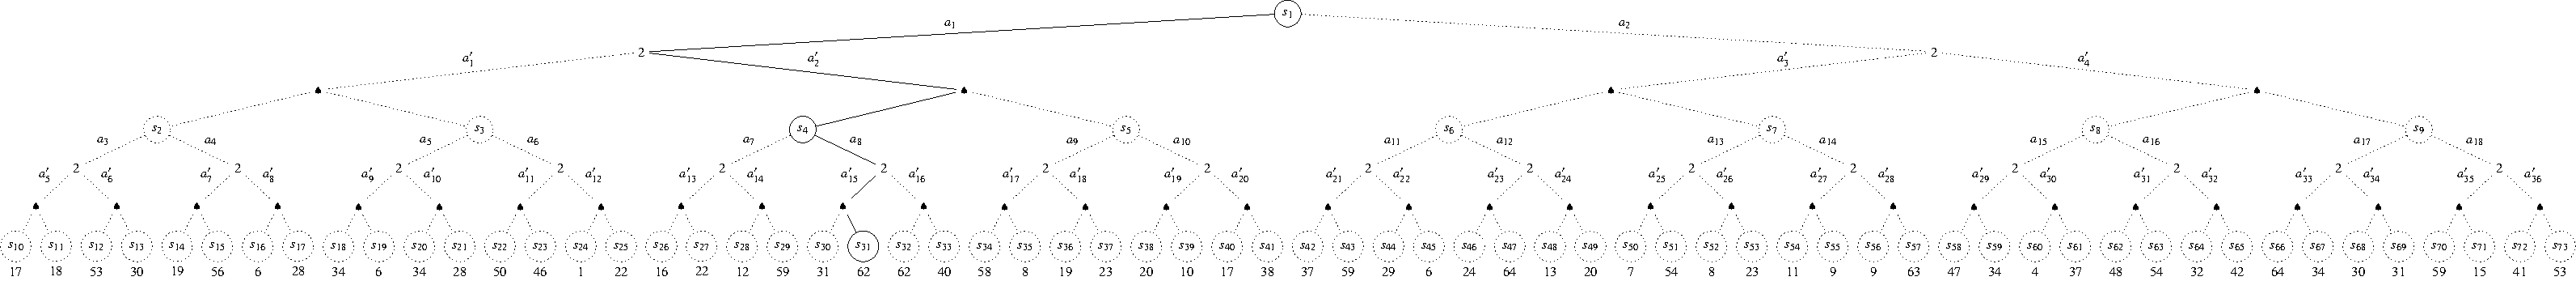
\includegraphics[width=\linewidth]{figures/tree-run}
    	\caption{Initial run with incomplete policy $\pi_{1} = \{ s_{1} \mapsto a_{1}, s_{4} \mapsto a_{8} \}$ such that $s_{31} \in G$}
    \end{subfigure}
    \begin{subfigure}{\linewidth}
        \centering
        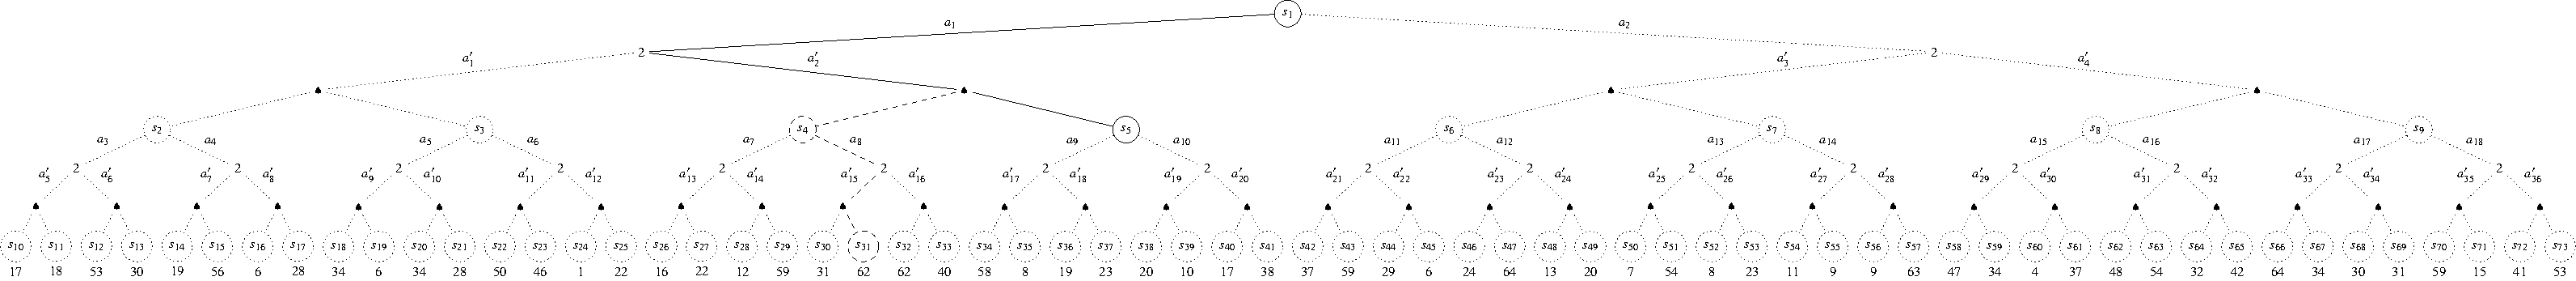
\includegraphics[width=\linewidth]{figures/tree-run-outcome}
    	\caption{Subsequent run with outcome not anticipated by $\pi_{1}$}
    \end{subfigure}
    \begin{subfigure}{\linewidth}
        \centering
        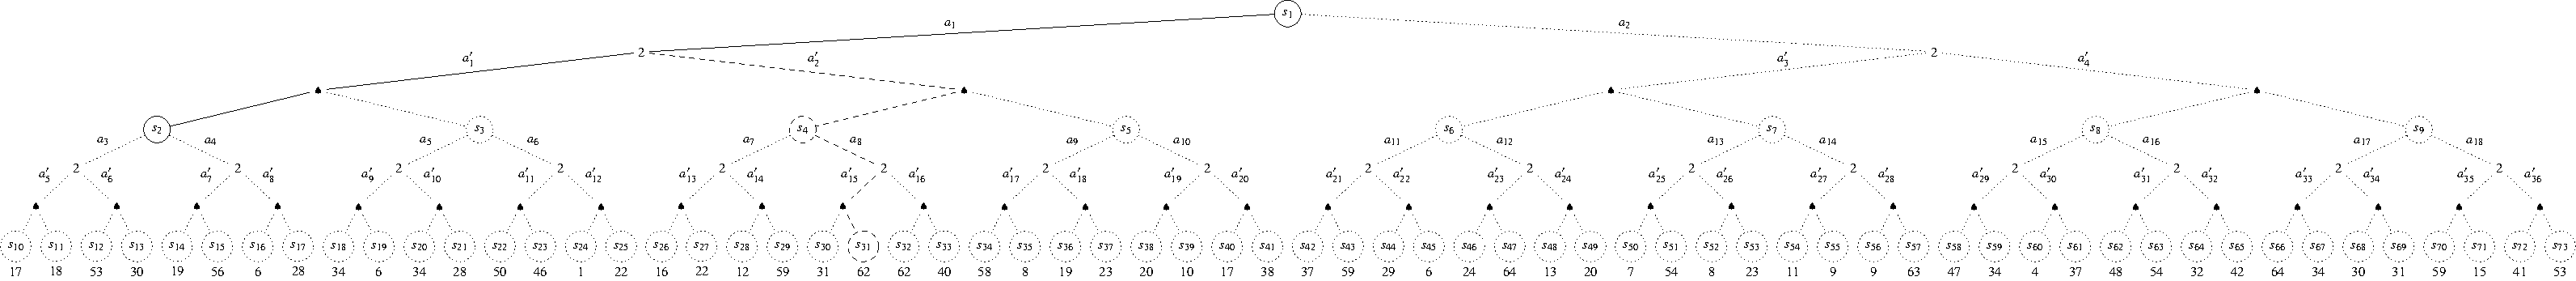
\includegraphics[width=\linewidth]{figures/tree-run-action}
    	\caption{Subsequent run with ego-action not anticipated by $\pi_{1}$}
    \end{subfigure}
    \begin{subfigure}{\linewidth}
        \centering
        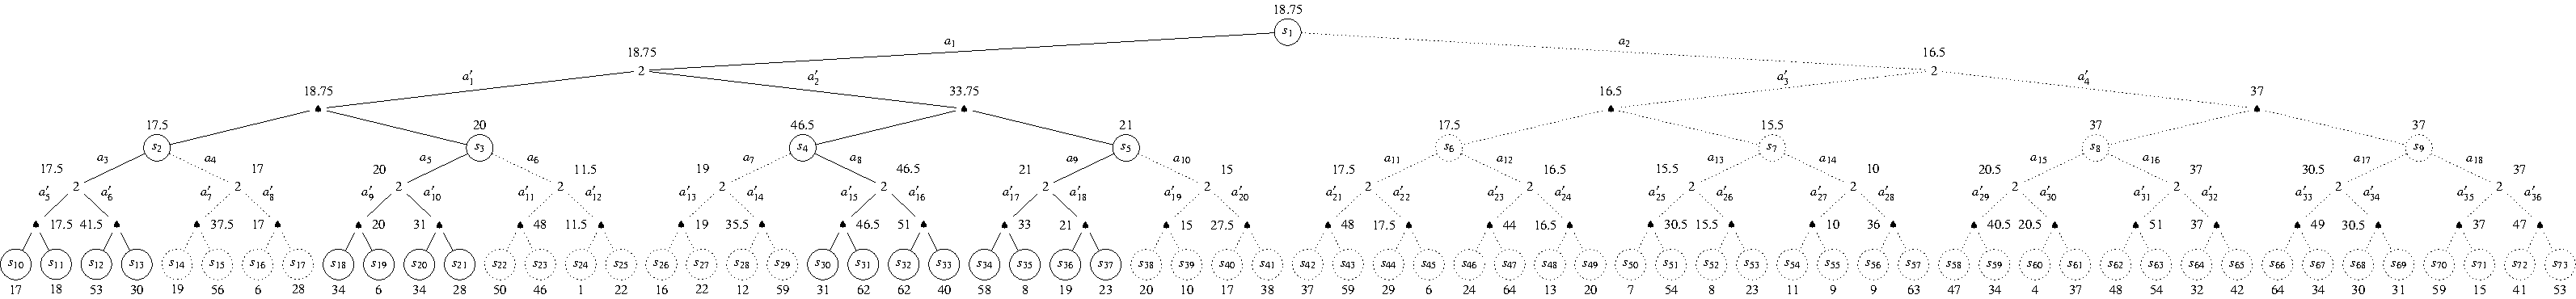
\includegraphics[width=\linewidth]{figures/tree-test}
    	\caption{Closed expectiminimax policy $\pi_{1}^{*} = \{ s_{1} \mapsto a_{1}, s_{2} \mapsto a_{4}, s_{3} \mapsto a_{5}, s_{4} \mapsto a_{7}, s_{5} \mapsto a_{10} \}$ such that $\{ s_{10}, \dots, s_{13}, s_{18}, \dots, s_{21}, s_{30}, \dots, s_{37}  \} \subseteq G$}
    \end{subfigure}
	\caption{SSP game with initial state $s_{1} \in S$ ($2$ denotes ego decision nodes, $\spadesuit$ denotes chance nodes, policies are stationary and pure)}
	\label{figure:game_tree}
\end{figure}
\end{landscape}

\begin{figure}[htbp]
	\footnotesize
    \centering
    \begin{forest}
        [$a_{1}$, draw, circle
            [{}, draw, circle, inner sep=0.25pt, fill, edge label={node[midway, above left]{$a_{1}'$}}
                [$a_{3}$, draw, circle, edge label={node[midway, above left]{$s_{2}$}}, edge={-latex}]
                [$a_{5}$, draw, circle, edge label={node[midway, above right]{$s_{3}$}}, edge={-latex}]
            ]
            [{}, draw, circle, inner sep=0.25pt, fill, edge label={node[midway, above right]{$a_{2}'$}}
                [$a_{8}$, draw, circle, edge label={node[midway, above left]{$s_{4}$}}, edge={-latex}]
                [$a_{9}$, draw, circle, edge label={node[midway, above right]{$s_{5}$}}, edge={-latex}]
            ]
        ]
    \end{forest}
	\caption{Visualisation of $\pi^{*}$ from Figure~\ref{figure:game_tree}}
	\label{figure:test}
\end{figure}

% \begin{lemma}\label{lemma:dead_ends}
%     Let $\mathcal{G}$ be a simulator-based testing game.
%     There exists a proper policy profile for $\mathcal{G}$ if and only if $\mathcal{G}$ does not exhibit dead-ends.
% \end{lemma}
%
% \begin{proof}[Proof Sketch]
%     The proof may be analogous to the proofs for SSPs~\cite{Kolobov:book:2012}, assuming it has not been proven already.
% \end{proof}
%
% \begin{definition}
%     A time-limited test generation game is a tuple $(\mathcal{G}, t_{\max})$ where $\mathcal{G}$ is a test generation game and $t_{\max} \in \mathbb{N}$ is a (finite-)horizon.
% \end{definition}
%
% \begin{proposition}
%     Let $(\mathcal{G}, t_{\max})$ be a time-limited test generation game.
%     There exists a proper policy profile for $(\mathcal{G}, t_{\max})$.
% \end{proposition}
%
% \begin{proof}[Proof Sketch]
%     The set of states $S$ can be translated into a new set of states $S' = S \times \{ 0, \dots, t_{\max} \}$.
%     The set of goal states $G$ can be translated into a new set of goal states $G' = \left( G \times \{ 0, \dots, t_{\max} \} \right) \cup \left( S \times \{ 0 \} \right)$.
%     The translated game $(\mathcal{G}', t_{\max})$ does not exhibit dead-ends because for any state $s \in S'$ there always exists a state $s' \in S \times \{ 0 \}$ such that $s'$ is reachable from $s$.
%     Thus, it follows from Lemma~\ref{lemma:dead_ends} that a proper policy profile for $G$ is guaranteed to exist.
% \end{proof}

% \begin{definition}
%     Let $\pi_{1}$ be a pure policy and $\omega \subseteq S$ be a (test) assertion.
%     An interesting test given $\pi_{1}$ and $\omega$ is a tuple $(s_{1}, \vect{\pi}_{-1})$ where $s_{1} \in S$ is an initial state and $\vect{\pi}_{-1}$ is a pure policy profile for the set of agents $N \setminus \{ 1 \}$ such that executing policy profile $(\pi_{1}, \vect{\pi}_{-1})$ in state $s_{1}$ leads to some state $s \in \omega$ within a finite number of timesteps.
% \end{definition}
%
% \begin{note}
%     Assertions could be generalised to sequences of states (e.g.\ using a termporal logic?) or to executions (e.g.\ with actions as events?).
% \end{note}
%
% \begin{note}
%     We assume that a mixed policy is always fixed to a pure policy by controlling the seed, but this means the test is only interesting with respect to that seed.
%     Is there a more general notion?
% \end{note}
%
% \begin{note}
%     How to \emph{repeat} a test when a different ego policy $\pi_{1}'$ may cause the assertion to be avoided altogether (e.g.\ by causing the agents to arrive in history $h \in H$ such that $\vect{\pi}_{-1}$ is undefined for $h$)?
% \end{note}
%
% \begin{definition}
%     Let $\pi_{1}$ be an ego policy, $\omega \subseteq S$ be a (test) goal, and $\theta \in (0, 1]$ be a probability threshold.
%     A satisficing test for $\pi_{1}$ with respect to $\omega$ is a tuple $(s_{1}, \vect{\pi}_{-1})$ where $s_{1} \in S$ is an initial state and $\vect{\pi}_{-1}$ is a pure policy profile for the set of agents $N \setminus \{ 1 \}$ such that executing policy profile $(\pi_{1}, \vect{\pi}_{-1})$ in state $s_{1}$ guarantees termination in some state $s \in \omega$ with probability $p \ge \theta$.
% \end{definition}
%
% \begin{note}
%     Do we need a reward function $R : S \times A \times S \to \mathbb{R}$ (where the objective is to maximise expected reward) or a non-negative cost function $C : S \times A \times S \to \mathbb{R}^{\ge 0}$ (where the objective is to minimise expected cost)?
%     Goal-oriented MDPs are typically defined with the latter.
% \end{note}
%
% \begin{note}
%     What is the appropriate (or required) domain of the reward function?
%     For example:
%     \begin{itemize}
%         \item $R' : S \times A \to \mathbb{R}$ such that $R'(s, a) = R(s, a, s') = R(s, a, s'')$ for all $s', s'' \in S$
%         \item $R' : S \to \mathbb{R}$ such that $R'(s) = R(s', a, s) = R(s'', a', s)$ for all $s', s'' \in S$ and all $a, a' \in A$
%     \end{itemize}
% \end{note}
%
% \begin{note}
%     Do we need a horizon $t_{\max} \in \mathbb{N}$ and/or discount factor $\gamma \in [0, 1)$?
%     For example:
%     \begin{itemize}
%         \item Finite-horizon Markov game with terminal states (horizon, terminal states, optional discount factor)
%         \item Infinite-horizon Markov game with terminal states (discount factor, terminal states, no horizon)
%         \item Indefinite-horizon Markov game (terminal states, no horizon, no discount factor)
%     \end{itemize}
%     How to ensure early terminations are preferred (i.e.\ that longer runs do not have the opportunity to acrue more value)? How to guarantee that proper policies exist?
% \end{note}
%
% \begin{table}[htbp]
%     \footnotesize
%     \centering
%     \caption{MDP Comparison}
%     \begin{tabular}{c c c l}
%         \toprule
%         $t_{\max} \in \mathbb{N}$ & $\gamma \in [0, 1)$ & $G \subseteq S$ & Class \\
%         \midrule
%         \xmark & \xmark & \xmark & --- \\
%         \xmark & \xmark & \cmark & Stochastic shortest path (SSP) \\
%         \xmark & \cmark & \xmark & Infinite-horizon (IFH) $\subset$ SSP \\
%         \xmark & \cmark & \cmark & \emph{IFH with absorbing states $\subset$ IFH} \\
%         \cmark & \xmark & \xmark & Finite-horizon (FH) $\subset$ SSP \\
%         \cmark & \xmark & \cmark & \emph{FH with absorbing states $\subset$ FH?} \\
%         \cmark & \cmark & \xmark & \emph{FH with decaying rewards $\subset$ FH?} \\
%         \cmark & \cmark & \cmark & \emph{FH with absorbing states and decaying rewards $\subset$ FH?} \\
%         \bottomrule
%     \end{tabular}
% \end{table}
%
% \begin{note}
%     How should time limits in RL-style episodes be interpreted?
%     Do they correspond to a finite-horizon or are they just a training mechanism~\cite{Pardo:ICML:2018}?
% \end{note}

\newpage
\section{Experiments}\label{section:case-study}

\begin{figure}[tbph]
    \scriptsize
    \begin{subfigure}{\linewidth}
        \centering
        \begin{forest}
            for tree={s sep=-1pt},
            if level=0{l sep+=10pt}{},
            [MAS
                [AV, label={above left:\emph{Design under Test}}
                    [Vehicle [Acceleration] [Steering]]
                ]
                [Agent
                    [Pedestrian [Acceleration] [Steering]]
                ]
                [$\dots$
                    [$\dots$ [$\dots$]]
                ]
                [Agent, label={above right:\emph{Test Generator}}
                    [Pedestrian [Acceleration] [Steering, edge label={node[midway,above  right]{~~~~~\emph{Simulator}}}]]
                ]
            ]
            \draw (-4.9, -0.25) [dotted] rectangle (-2, -1.2);
            \draw (-0.75, -0.25) [dotted] rectangle (4.6, -1.2);
            \draw (-4, -1.3) [dotted] rectangle (4.4, -2.5);
        \end{forest}
        \caption{single-body ego agent, $n$ single-body tester agents}
    \end{subfigure}
    \begin{subfigure}{\linewidth}
        \centering
        \begin{forest}
            for tree={s sep=-1pt},
            if level=0{l sep+=10pt}{},
            [MAS
                [AV, label={above left:\emph{Design under Test}}
                    [Vehicle [Acceleration] [Steering]]
                ]
                [Agent, label={above right:\emph{Test Generator}}
                    [Pedestrian [Acceleration] [Steering]]
                    [$\dots$ [$\dots$]]
                    [Pedestrian [Acceleration] [Steering, edge label={node[midway,above  right]{~~~~~\emph{Simulator}}}]]
                ]
            ]
            \draw (-4.15, -0.25) [dotted] rectangle (-1.25, -1.2);
            \draw (1, -0.25) [dotted] rectangle (3.85, -1.2);
            \draw (-3.3, -1.3) [dotted] rectangle (5.15, -2.5);
        \end{forest}
        \caption{single-body ego agent, $1$ multi-body tester agent}
    \end{subfigure}
    \caption{Agent-based test generation in \textsc{CAV-Gym:Pedestrians}}
\end{figure}

\begin{figure}[htbp]
    \centering
    \frame{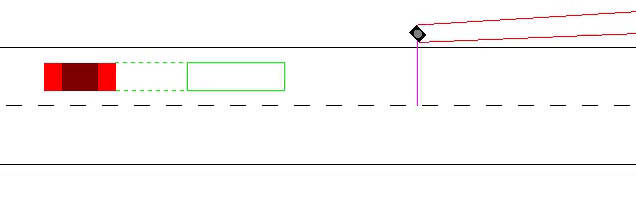
\includegraphics[width=\textwidth]{figures/cav-gym-cropped}}
    \caption{\textsc{CAV-Gym:Pedestrians}}
    \label{figure:cav-gym}
\end{figure}

\newpage
\bibliographystyle{plain}
\bibliography{agent-test-generation}

\newpage
\section*{Appendix: Kinematics}
A state is a tuple $s_{i} = (p_{i}, v_{i}, o_{i})$ where
$p_{i} \in \mathbb{R}^{2}$ is a position (point) denoted $p_{i} = (p_{i}^{x}, p_{i}^{y})$,
$v_{i} \in [v_{\min}, v_{\max}]$ is a velocity with $v_{\min}, v_{\max} \in \mathbb{R}^{\ge 0}$ such that $v_{\min} \le v_{\max}$,
and $o_{i} \in (-\pi, \pi]$ is an orientation (in radians).
Let $b \in \mathbb{R}^{\ge 0}$ be a wheelbase constant.
The positions of front and rear wheels $f_{i}, r_{i} \in \mathbb{R}^{2}$ in state $s_{i} = (p_{i}, v_{i}, o_{i})$ are:
\begin{align}
    f_{i}^{x} & = p_{i}^{x} + \frac{b}{2} \cos{o_{i}} \label{equation:kinematics_first} \\
    % & = \frac{b \cos{o_{i}}}{2} + p_{i}^{x} \\
    f_{i}^{y} & = p_{i}^{y} + \frac{b}{2} \sin{o_{i}} \\
    % & = \frac{b \sin{o_{i}}}{2} + p_{i}^{y} \\
    r_{i}^{x} & = p_{i}^{x} - \frac{b}{2} \cos{o_{i}} \\
    % & = \frac{-b \cos{o_{i}}}{2} + p_{i}^{x} \\
    r_{i}^{y} & = p_{i}^{y} - \frac{b}{2} \sin{o_{i}}
    % & = \frac{-b \sin{o_{i}}}{2} + p_{i}^{y}
\end{align}
A body has two effectors: throttle and steering.
An action is a tuple $a_{i} = (t_{i}, e_{i})$ where
$t_{i} \in [t_{\min}, t_{\max}]$ is a throttle with $t_{\min}, t_{\max} \in \mathbb{R}$ such that $t_{\min} \le t_{\max}$,
and $e_{i} \in [e_{\min}, e_{\max}]$ is a steering angle (in radians) with $e_{\min}, e_{\max} \in (-\frac{\pi}{2}, \frac{\pi}{2})$ such that $e_{\min} \le e_{\max}$.
Let $\lambda \in \mathbb{R}^{> 0}$ be a time resolution constant.
% Rotating point $a$ around pivot point $b$ by angle $\theta$ gives point $R_{b}^{\theta}(a)$ where:
% \begin{align}
%     R_{b}^{\theta}(a)^{x} & = b^{x} + (a^{x} - b^{x}) \cos{\theta} - (a^{y} - b^{y}) \sin{\theta} \\
%     % & = b^{x} + (a^{x} - b^{x}) \cos{\theta} + (-a^{y} + b^{y}) \sin{\theta} \\
%     R_{b}^{\theta}(a)^{y} & = b^{y} + (a^{x} - b^{x}) \sin{\theta} + (a^{y} - b^{y}) \cos{\theta}
%     % & = b^{y} + (a^{x} - b^{x}) \sin{\theta} + (a^{y} - b^{y}) \cos{\theta}
% \end{align}
If action $a_{i} = (t_{i}, e_{i})$ is executed in state $s_{i} = (p_{i}, v_{i}, o_{i})$ such that $e_{i} = 0$, then the successor state is $s_{i+1} = (p_{i+1}, v_{i+1}, o_{i+1})$ where:
\begin{align}
    p_{i+1}^{x} & = p_{i}^{x} + v_{i} \lambda \cos{o_{i}} \\
    p_{i+1}^{y} & = p_{i}^{y} + v_{i} \lambda \sin{o_{i}} \\
    v_{i+1} & = \min\{ v_{\max}, \max\{ v_{\min}, v_{i} + t_{i} \lambda \} \} \\
    o_{i+1} & = o_{i}
\end{align}
If action $a_{i} = (t_{i}, e_{i})$ is executed in state $s_{i} = (p_{i}, v_{i}, o_{i})$ such that $e_{i} \ne 0$, then the successor state is $s_{i+1} = (p_{i+1}, v_{i+1}, o_{i+1})$ where:
\begin{align}
    % c_{i}^{x} & = r_{i}^{x} + \frac{b}{\tan{e_{i}}} \cos{\left( o_{i} + \frac{\pi}{2} \right)} \\
    % & = \frac{-b \sin{o_{i}}}{\tan{e_{i}}} + r_{i}^{x} \\
    c_{i}^{x} & = r_{i}^{x} - \frac{b}{\tan{e_{i}}} \sin{o_{i}} \\
    % & = \frac{-b \sin{o_{i}}}{\tan{e_{i}}} - \frac{b \cos{o_{i}}}{2} + p_{i}^{x} = p_{i}^{x} - \frac{b}{2} \cos{o_{i}} - \frac{b}{\tan{e_{i}}} \sin{o_{i}} \\
    % c_{i}^{y} & = r_{i}^{y} + \frac{b}{\tan{e_{i}}} \sin{\left( o_{i} + \frac{\pi}{2} \right)} \\
    % & = \frac{b \cos{o_{i}}}{\tan{e_{i}}} + r_{i}^{y} \\
    c_{i}^{y} & = r_{i}^{y} + \frac{b}{\tan{e_{i}}} \cos{o_{i}} \\
    % & = \frac{-b \sin{o_{i}}}{2} + \frac{b \cos{o_{i}}}{\tan{e_{i}}} + p_{i}^{y} = p_{i}^{y} - \frac{b}{2} \sin{o_{i}} + \frac{b}{\tan{e_{i}}} \cos{o_{i}} \\
    \theta_{i} & = \frac{ \text{sgn}(e_{i}) v_{i} \lambda}{\sqrt{(c_{i}^{x} - p_{i}^{x})^{2} + (c_{i}^{y} - p_{i}^{y})^{2}}} \\
    & = \frac{\text{sgn}(e_{i}) 2 v_{i} \lambda}{\sqrt{b^{2} \left( 1 + \frac{4}{(\tan{e_{i}})^{2}} \right)}} \\
    p_{i+1}^{x} & = c_{i}^{x} + (p_{i}^{x} - c_{i}^{x}) \cos{\theta_{i}} - (p_{i}^{y} - c_{i}^{y}) \sin{\theta_{i}} \\
    % p_{i+1}^{x} & = R_{c_{i}}^{\theta_{i}}(p_{i})^{x} \\
    % p_{i+1}^{x} & = \frac{-b \sin{o_{i}}}{\tan{e_{i}}} + \frac{b \sin{(\theta_{i} + o_{i})}}{\tan{e_{i}}} - \frac{b \cos{o_{i}}}{2} + \frac{b \cos{(\theta_{i} + o_{i})}}{2} + p_x \\
    % & = \frac{b \sin{(\theta_{i} + o_{i})}}{\tan{e_{i}}} + \frac{b \cos{(\theta_{i} + o_{i})}}{2} + c_{i}^{x} \\
    % & = \frac{b}{\tan{e_{i}}} \sin{(\theta_{i} + o_{i})} + \frac{b}{2} \cos{(\theta_{i} + o_{i})} + c_{i}^{x} \\
    p_{i+1}^{y} & = c_{i}^{y} + (p_{i}^{x} - c_{i}^{x}) \sin{\theta_{i}} + (p_{i}^{y} - c_{i}^{y}) \cos{\theta_{i}} \\
    % p_{i+1}^{y} & = R_{c_{i}}^{\theta_{i}}(p_{i})^{y} \\
    % & = \frac{-b \sin{o_{i}}}{2} + \frac{b \sin{(\theta_{i} + o_{i})}}{2} + \frac{b \cos{o_{i}}}{\tan{e_{i}}} - \frac{b \cos{(\theta_{i} + o_{i})}}{\tan{e_{i}}} + p_y \\
    % & = \frac{b \sin{(\theta_{i} + o_{i})}}{2} - \frac{b \cos{(\theta_{i} + o_{i})}}{\tan{e_{i}}} + c_{i}^{y} \\
    % & = \frac{b}{2} \sin{(\theta_{i} + o_{i})} - \frac{b}{\tan{e_{i}}} \cos{(\theta_{i} + o_{i})} + c_{i}^{y} \\
    v_{i+1} & = \min\{ v_{\max}, \max\{ v_{\min}, v_{i} + t_{i} \lambda \} \} \\
    % o_{i+1} & = \arctantwo{ \left( R_{c_{i}}^{\theta_{i}}(f_{i})^{y} - R_{c_{i}}^{\theta_{i}}(r_{i})^{y}, R_{c_{i}}^{\theta_{i}}(f_{i})^{x} - R_{c_{i}}^{\theta_{i}}(r_{i})^{x} \right) } \\
    o_{i+1} & = \arctantwo{(\sin{(o_{i} + \theta_{i})}, \cos{(o_{i} + \theta_{i})})} \label{equation:kinematics_last}
\end{align}
The point $c_{i}$ is the centre of rotation for the given state-action pair (with non-zero steering action) and $\theta_{i}$ is the corresponding turn angle.
The body kinematics specified by Equations~\ref{equation:kinematics_first}--\ref{equation:kinematics_last} are illustrated in Figure~\ref{figure:kinematics}.
If action $a_{i} = (t_{i}, e_{i})$ is executed in state $s_{i} = (p_{i}, v_{i}, o_{i})$ such that $v_{i} > 0$ and results in successor state $s_{i+1} = (p_{i+1}, v_{i+1}, o_{i+1})$, then it follows that:
\begin{align}
    t_{i} & = \frac{v_{i+1} - v_{i}}{\lambda} \\
    \theta_{i} & = \arctantwo{(\sin{(o_{i+1} - o_{i})}, \cos{(o_{i+1} - o_{i})})} \\
    e_{i} & = \text{sgn}(\theta) \arctan{\left( 2 b \sqrt{\frac{\theta^{2}}{4 v_{i}^{2} \lambda^{2} - b^{2} \theta^{2}}} \right)} \label{equation:error}
    % & = -\arctan{\left( 2 b \frac{\sin{o_{i}} - \sin{o_{i+1}}}{b \cos{o_{i}} - b \cos{o_{i+1}} + 2 p_{i+1}^{x} - 2 p_{i}^{x}} \right)} \\
    % & = \arctan{\left( 2 b \frac{\cos{o_{i}} - \cos{o_{i+1}}}{b \sin{o_{i}} - b \sin{o_{i+1}} + 2 p_{i+1}^{y} - 2 p_{i}^{y}} \right)}
\end{align}
% The preferred method for calculating $e_{i}$ is Equation~\ref{equation:error} because empirical results have shown it to be less affected by floating point error.

\begin{figure}[htbp]
    \centering
    \footnotesize
    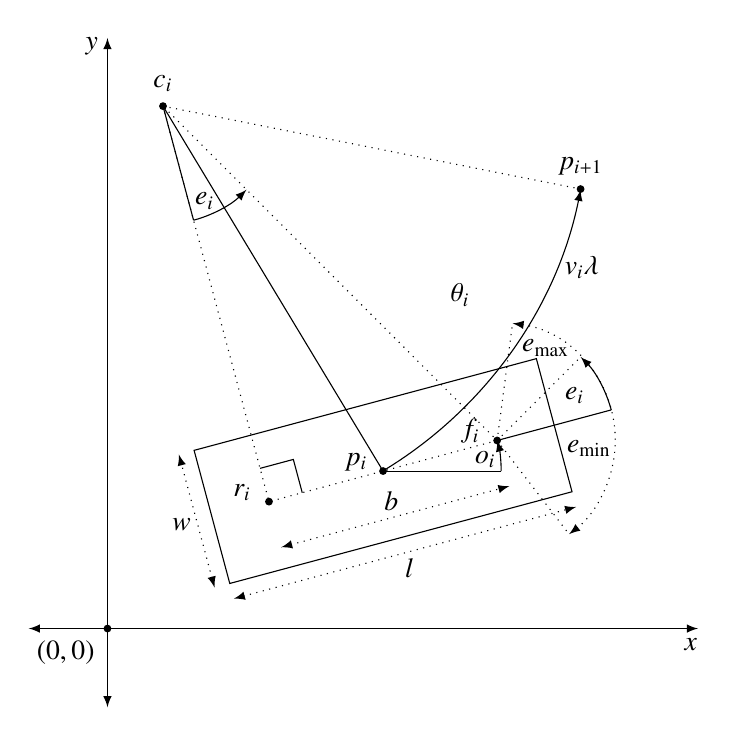
\begin{tikzpicture}
        \draw [latex-latex] (-1.0, 0.0) -- (7.5, 0.0); % X axis
        \draw [latex-latex] (0.0, -1.0) -- (0.0, 7.5); % Y axis
        \node at (7.4, -0.2) {$x$};
        \node at (-0.2, 7.4) {$y$};
        \node [circle, fill, inner sep=1pt, label={below left:$(0, 0)$}] at (0.0, 0.0) {};

        \begin{scope}[shift={(3.5, 2)}]
            \draw [-latex] (0.0, 0.0) ++(0:1.5) arc (0:15:1.5);
            \draw [-] (0.0, 0.0) -- (1.5, 0.0);
            \node at (1.3, 0.15) {$o_{i}$};
        \end{scope}

        \begin{scope}[shift={(3.5, 2)}, rotate around={15.0:(0.0, 0.0)}]
            \draw (-2.25, -0.875) rectangle ++(4.5, 1.75);
            \node [circle, fill, inner sep=1pt] at (0.0, 0.0) {};
            \node at (-0.3, 0.2) {$p_{i}$};
            \node [circle, fill, inner sep=1pt] at (1.5, 0.0) {};
            \node at (1.2, 0.2) {$f_{i}$};
            \node [circle, fill, inner sep=1pt] at (-1.5, 0.0) {};
            \node at (-1.8, 0.2) {$r_{i}$};
            \draw [latex-latex, dotted] (-1.5, -0.6) -- (1.5, -0.6);
            \node at (0.0, -0.4) {$b$};
            \draw [latex-latex, dotted] (-2.25, -1.075) -- (2.25, -1.075);
            \node at (0.0, -1.275) {$l$};
            \draw [latex-latex, dotted] (-2.45, -0.875) -- (-2.45, 0.875);
            \node at (-2.65, 0.0) {$w$};

            \draw (-1.5, 0.4375) -- (-1.0625, 0.4375) -- (-1.0625, 0);

            \node [circle, fill, inner sep=1pt, label={above:$c_{i}$}] at (-1.5, 5.2) {};
            \draw [dotted] (-1.5, 5.2) -- (-1.5, 0.0) -- (1.5, 0.0) -- (-1.5, 5.2);

            \begin{scope}[shift={(-1.5, 5.2)}, rotate around={-90.0:(0.0, 0.0)}]
                \draw [latex-] (0.0, 0.0) ++(30:1.5) arc (30:0:1.5);
                \draw [-] (0.0, 0.0) -- (1.5, 0.0);
                \node at (1.3, 0.2) {$e_{i}$};
            \end{scope}

            \node [circle, fill, inner sep=1pt, label={above:$p_{i+1}$}] at (3.35, 2.81) {};
            \draw [-] (-1.5, 5.2) -- (0.0, 0.0);
            \draw [-, dotted] (-1.5, 5.2) -- (3.35, 2.81);

            \begin{scope}[shift={(-1.5, 5.2)}, rotate around={-74.0:(0.0, 0.0)}]
                \draw [latex-] (0.0, 0.0) ++(47.67:5.41) arc (47.67:0:5.41);
                \node at (4, 2) {$\theta_{i}$};
                \node at (4.5, 3.5) {$v_{i} \lambda$};
            \end{scope}

            \begin{scope}[shift={(1.5, 0.0)}]
                \draw [latex-latex, dotted] (0.0, 0.0) ++(67.5:1.5) arc (67.5:-67.5:1.5);
                \draw [latex-] (0.0, 0.0) ++(30:1.5) arc (30:0:1.5);
                \draw [-] (0.0, 0.0) -- (1.5, 0.0);
                \draw [-, dotted, rotate around={30:(0, 0)}] (0, 0) -- (1.5, 0);
                \draw [dotted, rotate around={67.5:(0.0, 0.0)}] (0.0, 0.0) -- (1.5, 0.0);
                \draw [dotted, rotate around={-67.5:(0.0, 0.0)}] (0.0, 0.0) -- (1.5, 0.0);
                \node at (1.1, 0.3) {$e_{i}$};
                \node at (0.9, 0.975) {$e_{\max}$};
                \node at (1.1, -0.4) {$e_{\min}$};
            \end{scope}

        \end{scope}
    \end{tikzpicture}
    \caption{Body kinematics}
    \label{figure:kinematics}
\end{figure}

% \begin{note}[Problem]
%     Given state $s_{i}$ and target orientation $o_{g}$ such that $o_{g}$ is reachable from $s_{i}$ with a single action, find steering angle $e_{i}$ such that executing action $a_{i} = (t_{i}, e_{i})$ in $s_{i}$ results in successor state $s_{i+1} = (p_{i+1}, v_{i+1}, o_{i+1})$ where $o_{i+1} = o_{g}$ for any throttle $t_{i}$.
% \end{note}

\clearpage
\section*{Appendix: Algorithms}

\begin{note}[To do]
    Account for discretisation of continuous action spaces within each agent type (although, strictly speaking, \textsc{QLearningAgent} is the only agent type that requires a finite action space).
\end{note}

\begin{algorithm}[htbp]
	\caption{\textsc{Simulator}}
	\label{algorithm:simulation}
	\footnotesize
    \Persistent{environment $e$, agents $N = \{ 1, \dots, n \}$, terminator $\psi \subseteq S$}
    \Begin{
        \ForEach{episode}{
            $s \leftarrow$ reset $e$\;
            \ForEach{timestep}{
                $\vect{a} \leftarrow \left( \textsc{ChooseAction}_{1}(s), \dots, \textsc{ChooseAction}_{n}(s) \right)$\;
                $\vect{r}, s' \leftarrow$ execute $\vect{a}$ in $e$\;
                \ForEach{agent $i \in N$}{$\textsc{ProcessFeedback}_{i}(s, a_{i}, r_{i}, s')$}
                \leIf{$s' \in \psi$}{\Break}{$s \leftarrow s'$}
            }
        }
    }
\end{algorithm}

\begin{algorithm}[htbp]
	\caption{\textsc{RandomAgent}}
	\label{algorithm:random_agent}
	\footnotesize
    \Persistent{exploration rate $\epsilon \in [0, 1]$}
    \Function{$\textsc{ChooseAction}(s)$}{
        \WithProbability{$\epsilon$}{
            \Return random choice from $A(s)$
        }
        \Return $\varnothing$
    }
\end{algorithm}

\begin{algorithm}[htbp]
	\caption{\textsc{ProgrammedRandomAgent}}
	\label{algorithm:random_constrained_agent}
	\footnotesize
    \Persistent{programmed behaviour $\pi : S \to A$, terminator $\psi \subseteq S$, exploration rate $\epsilon \in [0, 1]$}
    \Function{$\textsc{ChooseAction}(s)$}{
        \If{$\pi$ is active}{
            \leIf{$s \in \psi$}{set $\pi$ as inactive}{\Return $\pi(s)$}
        }
        \WithProbability{$\epsilon$}{
            set $\pi$ as active\;
            \Return $\pi(s)$
        }
        \Return $\varnothing$
    }
\end{algorithm}

\begin{algorithm}[htbp]
	\caption{\textsc{ProgrammedReactiveAgent}}
	\label{algorithm:proximity_agent}
	\footnotesize
    \Persistent{programmed behaviour $\pi : S \to A$, trigger $\varphi \subseteq S$, terminator $\psi \subseteq S$}
    \Function{$\textsc{ChooseAction}(s)$}{
        \If{$\pi$ is active}{
            \leIf{$s \in \psi$}{set $\pi$ as inactive}{\Return $\pi(s)$}
        }
        \If{$s \in \varphi$}{
            set $\pi$ as active\;
            \Return $\pi(s)$
        }
        \Return $\varnothing$
    }
\end{algorithm}

\begin{algorithm}[htbp]
	\caption{\textsc{ProgrammedElectionAgent}}
	\label{algorithm:election_agent}
	\footnotesize
    \Persistent{programmed behaviour $\pi : S \to A$, terminator $\psi \subseteq S$, coordinator $c$}
    \Function{$\textsc{ChooseAction}(s)$}{
        \If{$\pi$ is active}{
            \leIf{$s \in \psi$}{set $\pi$ as inactive}{\Return $\pi(s)$}
        }
        \If{elected by $c$}{
            set $\pi$ as active\;
            \Return $\pi(s)$
        }
        \Return $\varnothing$
    }
\end{algorithm}

\begin{algorithm}[htbp]
	\caption{\textsc{QLearningAgent}}
	\label{algorithm:qlearning_agent}
	\footnotesize
    \Persistent{learning rate $\alpha \in [0, 1]$, discount factor $\gamma \in [0, 1)$, exploration rate $\epsilon \in [0, 1]$,\newline
    feature $f_{j} : S \times A \to \mathbb{R}$ with weight $w_{j} \in \mathbb{R}$ for $j = 1, \dots, m$}
    \Function{$\textsc{ChooseAction}(s)$}{
        \WithProbability{$\epsilon$}{
            \Return random choice from $A(s)$
        }
        \Return random choice from $\argmax_{a \in A(s)} \textsc{QValue}(s, a)$
    }
    \Procedure{$\textsc{ProcessFeedback}(s, a, r, s')$}{
        $q \leftarrow \left( r + \gamma \cdot \max_{a' \in A(s')} \textsc{QValue}(s', a') \right) - \textsc{QValue}(s, a)$\;
        \ForEach{feature $f_{j}$}{$w_{j} \leftarrow w_{j} + \alpha \cdot q \cdot f_{j}(s, a)$}
    }
    \Function{$\textsc{QValue}(s, a)$}{
        \Return $\sum_{j = 1}^{m} f_{j}(s, a) \cdot w_{j}$
    }
\end{algorithm}

\end{document}
